\section{Learned score: it breaks, and the corrected sampler fixes it}
\label{sec:learned}

\paragraph*{Setup.}
We train score networks by denoising score matching~\cite{vincent2011dsm,hyvarinen2005score} in the $\varepsilon$ form with unit weight, following Ref.~\cite{namba2026learned}.
Each is a multilayer perceptron with three hidden layers of 128 SiLU units, trained with Adam and cosine decay for 300\,000 steps; the exponential moving average of its weights is used for sampling.
The input is preconditioned by the data moments carried by the flow, in the spirit of Ref.~\cite{karras2022edm}.
Half of each batch is drawn with $\sigma\in[\smin,10\smin]$.
The training set holds $200\,000$ samples.
Each network takes about 23 minutes on one CPU core, and we train two per setting: B, C, and D (D is the setup of Sec.~\ref{sec:exact}, $\smin=s/16$).
Every learned-score run is paired with an exact-score run that uses the same prior draw and Brownian increments, so the difference $\Delta=L_{\rm learned}-L_{\rm exact}$ isolates the effect of the score error (two networks $\times$ three seeds, $N=20\,000$, $h\approx0.002$).
The success criteria were fixed before any results of these runs were available.

\begin{observation}[the clipped sampler breaks as much as with the exact score]
\label{obs:learned-break}
The paired shrinkage of \Sa{} relative to \Sb{} is $-0.1170$ (learned) against $-0.1167$ (exact) in setting B, $-0.2093$ against $-0.2069$ in C, and $-0.0191$ against $-0.0188$ in D.
The ratios are $1.00$, $1.01$ and $1.02$ (Table~\ref{tab:learned}).
\end{observation}

\begin{observation}[the corrected sampler fixes it]
\label{obs:learned-fix}
The learned score moves the corrected sampler by $\Delta_{\rm ii}=+0.4\%$ (B) and $+0.7\%$ (C), about one thirtieth of the shrinkage it removes.
In D, where the score error near $\smin$ is $11.8\%$, $\Delta_{\rm ii}=+3.9\%$, twice the threshold effect ($1.9\%$).
Even there, the paired difference between \Sa{} and \Sb{} is unchanged.
\end{observation}

The score error thus \emph{adds} to the threshold effect, widening \Sa{} and \Sb{} by the same amount ($\Delta_{\rm i}\approx\Delta_{\rm ii}$), and does not interact with it.
Proposition~\ref{prop:difference} gives the reason: only $\tfrac12\Gm\delta$ distinguishes the two samplers.
The learned scores are least accurate exactly where Observation~\ref{obs:local} says the damage is made: the relative error rises steeply as $\sigma\to\smin$ (to 47\% at $\smin$ in D) [Fig.~\ref{fig:learned}(c)].
Across training checkpoints, $\Delta_{\rm i}$ and $\Delta_{\rm ii}$ decrease monotonically with this error [Fig.~\ref{fig:learned}(b)].

\begin{table}[t]
\caption{Learned against exact score (two networks $\times$ three seeds). $e$: relative score error averaged over $\sigma\in[\smin,2\smin]$. Paired: $L$ of \Sa{} relative to \Sb{}. $\Delta$: learned minus exact, in units of $100L$.}
\label{tab:learned}
\begin{ruledtabular}
\begin{tabular}{lccccc}
 & $e$ & paired, learned (exact) & ratio & $\Delta_{\rm ii}$ & $\Delta_{\rm iii}$ \\
\hline
B & $0.09\%$ & $-0.1170$ ($-0.1167$) & $1.00$ & $0.4$ & $2.7$ \\
C & $1.2\%$ & $-0.2093$ ($-0.2069$) & $1.01$ & $0.7$ & $0.8$ \\
D & $11.8\%$ & $-0.0191$ ($-0.0188$) & $1.02$ & $3.9$ & diverges \\
\end{tabular}
\end{ruledtabular}
\end{table}

\begin{observation}[the probability-flow ODE is fragile]
\label{obs:ode}
With the same networks the ODE deviates more than \Sb{}: $\Delta_{\rm iii}=2.7\%$ in B.
Early in training it doubles the variance or more, and in D $16/24\,000$ trajectories diverge, which dominates the variance.
No divergence occurs with the exact score, or with the learned score in \Sa{} or \Sb{}.
\end{observation}

\begin{observation}[score weighting]
\label{obs:weighting}
Weighting the loss by $(\smin/\sigma)^2$, the ``score'' weighting of Ref.~\cite{namba2026learned}, does not help in D.
The error near $\smin$ stays at $10.6\%$.
Because $\sigma$ spans a factor of $8000$, the weight falls to $\sim10^{-8}$ at large $\sigma$, where the score is then left nearly unlearned.
All three samplers diverge within the first $\sim50$ reverse steps ($18$ of $18$ runs).
This failure was predicted before the runs.
\end{observation}

\begin{figure*}[t]
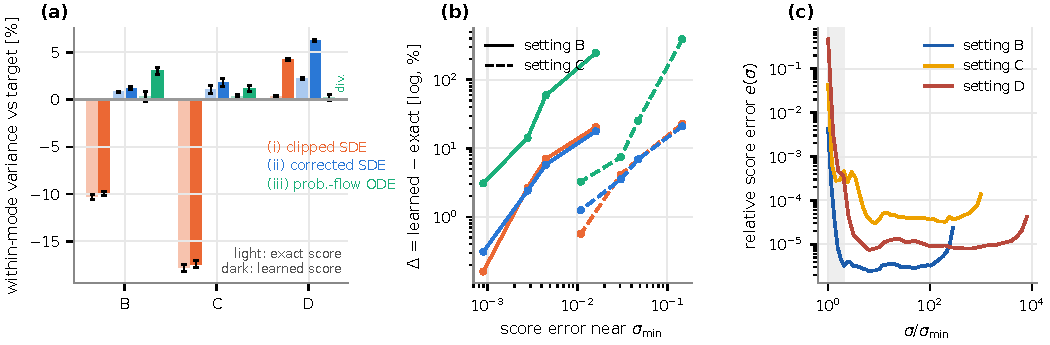
\includegraphics[width=\textwidth]{figures/fig3_learned}
\caption{Learned score.
(a) Within-mode variance against target for the three samplers, with the exact (light) and learned (dark) score, at step $h\approx0.002$ (the small positive values of \Sb{} with the exact score are discretization error, which vanishes under step extrapolation).
(b) $\Delta$ (learned minus exact) against the score error near $\smin$, over training checkpoints (10k--300k steps, one network and seed).
(c) Relative score error $e(\sigma)$ of the final networks; the shaded band is $[\smin,2\smin]$.}
\label{fig:learned}
\end{figure*}
